\documentclass[12pt,oneside]{book}
\usepackage{lipsum}
\usepackage[dvips,xetex]{graphicx} 
\usepackage[top=3cm, bottom=3cm, left=2.5cm, right=4cm]{geometry}
\geometry{a4paper}
\graphicspath{{images/}}
\usepackage{fancyhdr}
\pagestyle{fancy}
\cfoot{\thepage}
\lhead{}
\usepackage[DIV=14,BCOR=2mm,headinclude=true,footinclude=false]{typearea}
\usepackage[T1]{fontenc}
\usepackage[utf8]{inputenc}
\usepackage{lmodern}
\usepackage{color}
\usepackage[extrafootnotefeatures]{xepersian}
\linespread{1.5}
\selectfont
\renewcommand{\footnotesize}{\normalsize}
\settextfont{Vazir}
\setlatintextfont{TimesNewerRoman-Regular}
\title{\textbf{خودآموز زبان C}}
\author{سعید}
\begin{document}
\paragraphfootnotes
\begin{figure}
\centering
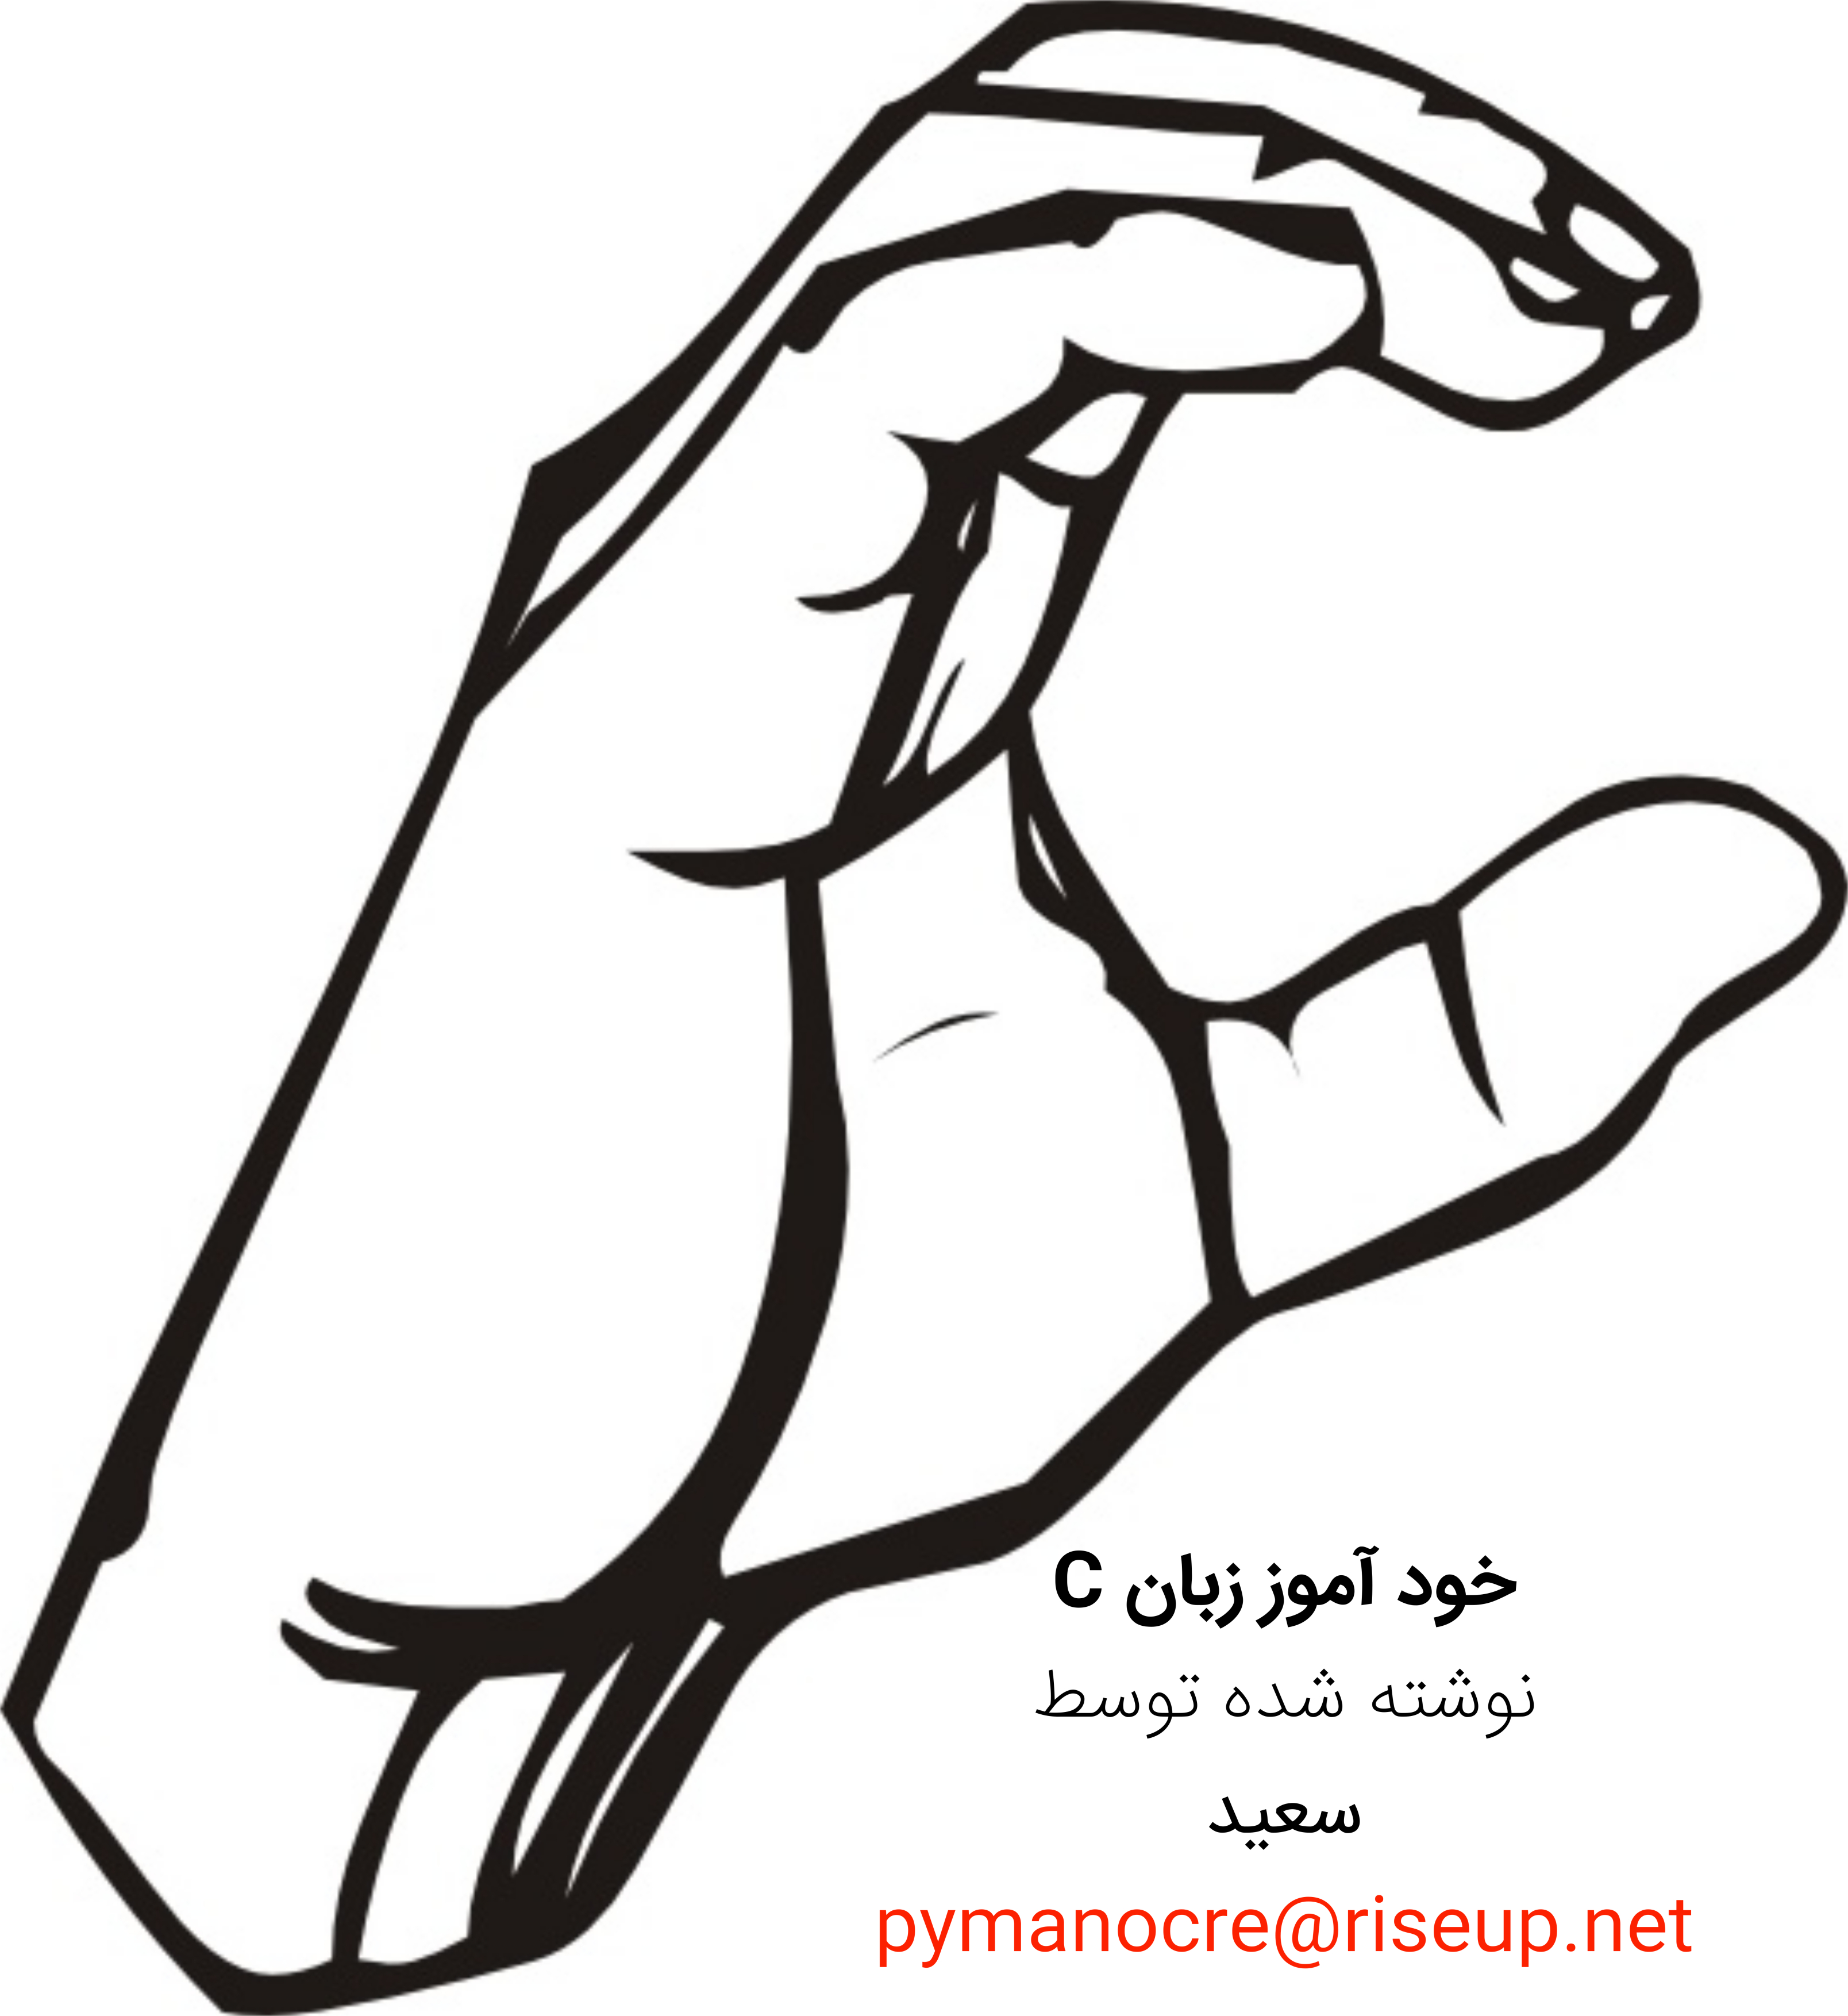
\includegraphics[width=150mm]{c_artwork}
\end{figure}
\clearpage\maketitle
\thispagestyle{empty}
\pagenumbering{Alph}
\tableofcontents
\addcontentsline{toc}{chapter}{پیشگفتار}
\chapter*{پیش‌گفتار}
  در اینجا ما امتحان میکنیم.

\pagenumbering{arabic}
\part{مفاهیم و تعاریف}
\chapter{تعریف برنامه‌نویسی}
\section{برنامه‌نویسی و زبان برنامه‌نویسی}
\section{برنامه و اسکریپت}

\chapter{تاریخچه زبان C}

\chapter{استاندارهای C}
\section{استاندارد ANSI/ISO}
\section{استاندارد C99}
\section{استاندارد C11}
\section{استاندارد C18}

\chapter{ویژگی‌های زبان C}
\section{طراحی}
\subsection{ساختار بالا به پایین}
\subsection{کتابخانه‌های استاندارد}
\subsection{برنامه‌نویسی ماژولار}
\section{بهینگی}
\section{قابلیت حمل}
\section{قدرت و انعطاف‌پذیری}
\section{آزادی}

\end{document}
